% interacttfssample.tex
% v1.05 - August 2017

\documentclass[]{interact}

\usepackage{epstopdf}% To incorporate .eps illustrations using PDFLaTeX, etc.
%\usepackage[caption=false]{subfig}% Support for small, `sub' figures and tables
%\usepackage[nolists,tablesfirst]{endfloat}% To `separate' figures and tables from text if required

%\usepackage[doublespacing]{setspace}% To produce a `double spaced' document if required
%\setlength\parindent{24pt}% To increase paragraph indentation when line spacing is doubled
%\setlength\bibindent{2em}% To increase hanging indent in bibliography when line spacing is doubled

\usepackage[numbers,sort&compress]{natbib}% Citation support using natbib.sty

\usepackage{xcolor}
\usepackage{amsthm}
\usepackage{subfloat}
\usepackage{graphicx}
\usepackage{caption}
\usepackage{subcaption}
\usepackage{multirow}
\usepackage{amsmath, amssymb, amsfonts}
\usepackage{graphicx}
\usepackage{hyperref}
%\usepackage{cite}
\usepackage{lipsum}
\usepackage{listings}
\usepackage{booktabs}
\usepackage{xcolor}
\usepackage{amsthm}
\usepackage{caption}
\usepackage{listings}
\usepackage{algpseudocode}
\usepackage{algorithm}
\newcommand{\vect}{\operatorname{vec}}
\bibpunct[, ]{[}{]}{,}{n}{,}{,}% Citation support using natbib.sty
\renewcommand\bibfont{\fontsize{10}{12}\selectfont}% Bibliography support using natbib.sty
\setlength{\parindent}{0pt}
\hypersetup{
    colorlinks=true,
    linkcolor=blue,
    filecolor=magenta,      
    urlcolor=cyan,
    pdftitle={IPNSDP User Manual},
    pdfauthor={Alemseged G. Weldeyesus},
    pdfsubject={Nonlinear Semidefinite Programming Solver}
}

\lstset{
    language=Matlab,
    basicstyle=\ttfamily\small,
   % keywordstyle=\color{blue}\bfseries,
    commentstyle=\color{green!50!black}\itshape,
  % stringstyle=\color{red},
    showstringspaces=false,
    identifierstyle=\color{black},
    numberstyle=\tiny\color{gray},
    numbers=left,
    stepnumber=0,
    numbersep=11pt,
    tabsize=1,
    breaklines=true,
    breakatwhitespace=true,
    captionpos=b,
    frame=single,
    frameround=auto,
    framesep=0pt,
    rulesepcolor=\color{gray!20!white},
    escapeinside={(*@}{@*)},
    morekeywords={function, end, if, else, struct, cell, import, casadi, disp, fprintf}
}

\theoremstyle{plain}% Theorem-like structures provided by amsthm.sty
\newtheorem{theorem}{Theorem}[section]
\newtheorem{lemma}[theorem]{Lemma}
\newtheorem{corollary}[theorem]{Corollary}
\newtheorem{proposition}[theorem]{Proposition}

\theoremstyle{definition}
\newtheorem{definition}[theorem]{Definition}
\newtheorem{example}[theorem]{Example}

\theoremstyle{remark}
\newtheorem{remark}{Remark}
\newtheorem{notation}{Notation}

\begin{document}

\articletype{Research article}% Specify the article type or omit as appropriate

\title{IPNSDP: A Solver for Nonlinear Semidefinite Programming with Automatic Differentiation and Chordal Decomposition}

\author{
\name{ A.~G. Weldeyesus\textsuperscript{a} and M.~F. Anjos\textsuperscript{a,b}}
\affil{\textsuperscript{a} \thanks{M.~F. Anjos. Email: Miguel.F.Anjos@ed.ac.uk}  School of Mathematics
and Maxwell Institute for Mathematical Sciences
The University of Edinburgh, Peter Guthrie Tait Road, Edinburgh EH9 3FD, 
United Kingdom; \textsuperscript{b}
GERAD, 3000, chemin de la Côte-Sainte-Catherine, Montréal, QC H3T 2A7, Canada.}
}

\maketitle

\begin{abstract}
This paper introduces IPNSDP, a MATLAB solver for general Nonlinear Semidefinite Programming (NSDP) based on a second-order interior point method. Unlike linear SDP solvers, existing NSDP solvers are very limited and often require users to provide difficult manual derivatives or rely on other modeling interfaces. IPNSDP addresses this by directly integrating with CasADi for automatic differentiation, significantly reducing user effort. For large-scale and structured sparse problems, it supports chordal decomposition, replacing large positive semidefinite constraints with smaller ones, enhanced by a merging strategy that combines submatrices with significant overlap to improve computational efficiency. By integrating automatic differentiation with optimized decomposition, IPNSDP offers a user-friendly scalable solution for a broad class of NSDP problems.
\end{abstract}

\begin{keywords}
Nonlinear semidefinite programming;  interior point methods; tables; mathematics; Chordal decomposition

\end{keywords}


\section{Introduction}

This paper presents IPNSDP, a MATLAB-based general-purpose solver to tackle a broad class of Nonlinear Semidefinite Programming (NSDP) problems. IPNSDP implements a second-order primal-dual interior point method and leverages automatic differentiation from CasADi to automate the computation of all required derivatives. In addition, the solver exploits chordal decomposition to efficiently handle large-scale sparse and structured matrix inequalities, significantly enhancing computational scalability.

NSPD generalizes the well-established framework of linear semidefinite programming to accommodate nonlinear objectives and constraints. NSDP arises in diverse application areas, including finance~\cite{higham2002computing}, control theory~\cite{Kocvara_control}, structural optimization~\cite{Kocvara2002, Weldeyesus2024}, polynomial optimization~\cite{parrilo2003semidefinite}, machine learning~\cite{Konno2003} etc. However, the non-linear nature of these problems introduces challenges, particularly in derivative evaluation, which often involves a difficult matrix calculus.

While several robust and efficient solvers exist for linear semidefinite programming, such as SDPT3~\cite{TohToddTutuncu1999}, SeDuMi~\cite{Sturm1999}, and MOSEK~\cite{mosek},  the tools and methods available for solving NSDPs remain relatively limited~\cite{HiroshiYamashita2015}, although recent approaches based on sequential quadratic programming have been developed, for example, as proposed in~\cite{Kosuke2023}. In most cases, solvers for NSDPs such as PENNON~\cite{pennon} and PENLAB~\cite{penlab} have been used. These solvers are implemented using the augmented Lagrangian method and can handle a broad class of NSDPs. However, users are required to manually implement derivatives of nonlinear functions involving matrix calculus or to rely on interfaces such as YALMIP~\cite{yalmip}.

 We developed IPNSDP as alternative for tackling NSDPs, particularly those exhibiting convexity. It combines a user-friendly MATLAB interface with CasADi~\cite{Andersson2019} as automatic differentiation engine. Therefore, users are only required to define the objective and constraint functions. All relevant first- and second-order derivatives are computed internally. This substantially reduces the modeling complexity of NSDPs and simplifies the application of NSDP methods to practical problems.

Furthermore, IPNSDP employs a well-known and efficient chordal decomposition technique~\cite{Fukuda2001, KimKMY11, Lieven2015, ZHENG2021243} to transform positive semidefinite constraints on large, structured sparse matrices into multiple positive semidefinite constraints on smaller submatrices. Such structured and sparse NSDPs commonly arise in applications such as structural optimization~\cite{Kocvara21, Weldeyesus2024}. To further enhance the efficiency of this decomposition, a graph-based clique merging strategy~\cite{GARSTKA2020} is utilized to combine submatrices with significant overlap. The overall processes of decomposition and merging are all customizable by the user through the options included in the solver. This combined approach substantially reduces the computational cost  and improves the numerical tractability of many  sparse and structured NSDPs.

The paper is organized as follows. Section~\ref{sec:prob} describes the general NSDP problem formulation addressed by IPNSDP. Section~\ref{sec:chord_decomp} explains the theoretical background and implementation of chordal decomposition and clique merging. The implemented primal-dual interior point method and its associated parameters are detailed in Section~\ref{sec:IPM}. Section~\ref{sec:usage_prob} describes how to use the solver, including problem setup and customization options. Several examples from the literature are solved in Section~\ref{sec:eg}. Finally, concluding remarks are provided in Section~\ref{sec:conc}.


\section{Problem Formulation}\label{sec:prob}
The solver IPNSDP addresses a general NSDP problem of the form:
\begin{equation}\label{eq:genform_explicit}
\begin{aligned}
& \min_{X_k \in \mathbb{S}^{d_k},\, u \in \mathbb{R}^n} \quad && f(X,u) \\
& \text{subject to}
& & \sum_{k=1}^{m_X} \langle A_{11,i}^{(k)}, X_k \rangle + A_{12,i} u = b_{1,i}, \quad i=1,\dots,n_1 \\
& & & \sum_{k=1}^{m_X} \langle A_{21,j}^{(k)}, X_k \rangle + A_{22,j} u \leq b_{2,j}, \quad j=1,\dots,n_2 \\
& & & c_1(X,u) = 0 \\
& & & c_2(X,u) \leq 0 \\
& & & \mathcal{A}_s(X,u) \succeq 0, \quad s=1,\dots,n_{psd} \\
& & & \underline{u} \leq u \leq \bar{u} \\
& & & \underline{\rho}_k I_{d_k} \preceq X_k \preceq \bar{\rho}_k I_{d_k}, \quad k=1,\dots,m_X.
\end{aligned}
\end{equation}

The problem involves two sets of decision variables. The first one is a tuple of symmetric matrices $X = (X_1, \ldots, X_{m_X})$, where each matrix $X_k$ is in the space $\mathbb{S}^{d_k}$ and is constrained to be positive semidefinite. The constants \( \underline{\rho}_k \geq 0 \) and  \( \bar{\rho}_k \) define the lower and upper bound on the eigenvalues of \( X_k \), and \( I_{d_k} \) denotes the \( d_k \times d_k \) identity matrix. The other variable is a vector $u \in \mathbb{R}^n$ with \(\underline{u}\) and \(\bar{u}\) its lower and upper bounds. The objective function \( f: \mathbb{S} \times \mathbb{R}^n \to \mathbb{R} \) and the nonlinear constraint functions \( c_1: \mathbb{S} \times \mathbb{R}^n \to \mathbb{R}^{q_1} \) and \( c_2: \mathbb{S} \times \mathbb{R}^n \to \mathbb{R}^{q_2} \) are assumed to be sufficiently smooth. The linear constraints involve the trace inner product,
\begin{equation}\label{eq:inner_pro}
\langle A, X \rangle := \operatorname{trace}(A  X).
\end{equation}
with symmetric coefficient matrices $A_{11,i}^{(k)} \in \mathbb{S}^{d_k}$ and $A_{21,j}^{(k)} \in \mathbb{S}^{d_k}$ for $i = 1, \ldots, n_1$ and $j = 1, \ldots, n_2$, respectively.
Moreover, $A_{12,i} \in \mathbb{R}^{1 \times n}$ and $A_{22,j} \in \mathbb{R}^{1 \times n}$, and $b_{1,i}$ and $b_{2,j}$ are right hand side constants. Each map $\mathcal{A}_s : \mathbb{S} \times \mathbb{R}^n \to \mathbb{S}^{t_s}$ produces a symmetric  positive matrix of size $t_s \times t_s$.

\begin{remark}
While Problem~\eqref{eq:genform_explicit} includes explicit linear constraints, it may be simpler for the user to embed them within the nonlinear constraint function for IPNSDP. 
\end{remark}

Note that if we replace the objective function \( f(X,u) \) with a linear function and remove the nonlinear constraints in Problem~\eqref{eq:genform_explicit}, the formulation reduces to a well-known primal linear SDP formulation:

\begin{equation}\label{eq:genform_linear}
\begin{aligned}
& \underset{X_k \in \mathbb{S}^{d_k},\, u \in \mathbb{R}^n}{\text{minimize}}
& & \sum_{k=1}^{m_X} \langle C_k, X_k \rangle + c_u^T u \\
& \text{subject to} \\
& & & \sum_{k=1}^{m_X} \langle A_{11,i}^{(k)}, X_k \rangle + A_{12,i} u = b_{1,i}, \quad i = 1, \dots, n_1 \\
& & & \sum_{k=1}^{m_X} \langle A_{21,j}^{(k)}, X_k \rangle + A_{22,j} u \leq b_{2,j}, \quad j = 1, \dots, n_2 \\
& & & \underline{u} \leq u \leq \bar{u} \\
& & & \underline{\rho}_k I_{d_k} \preceq X_k \preceq \bar{\rho}_k I_{d_k}, \quad k=1,\dots,m_X.
\end{aligned}
\end{equation}


Although the linear SDP Problem~\eqref{eq:genform_linear} can be solved using IPNSDP, we generally recommend  other efficient solvers specifically designed for linear SDPs. IPNSDP is primarily intended as an alternative solver for NSDPs. 

\section{Chordal decomposition and merging}\label{sec:chord_decomp}
This section provides a brief overview of the chordal decomposition and merging strategy implemented in IPNSDP. The decomposition technique transforms each positive semidefinite constraint on a large  sparse matrices into several positive semidefinite constraints on smaller submatrices. The  effectiveness of this decomposition technique can be improved by combining submatrices with significant overlap.  For a detailed theoretical discussion of chordal decomposition and merging techniques, we refer the reader to~\cite{Fukuda2001, KimKMY11, Lieven2015, ZHENG2021243,  GARSTKA2020}.

We closely follow the presentation and content of Section 3 of~\cite{Weldeyesus2024}.


The chordal decomposition originates from graph theory, where the relevant definitions are as follows. An undirected graph \( G = (\mathcal{V}, \mathcal{E}) \) is defined by a finite set of vertices \( \mathcal{V} = \{1, \dots, n\} \) and a set of undirected edges \( \mathcal{E} \subseteq \mathcal{V} \times \mathcal{V} \), where \( (\nu_i, \nu_j) \in \mathcal{E} \) implies \( (\nu_j, \nu_i) \in \mathcal{E} \). A \emph{path} in \( G \) is a sequence of vertices \( \{\nu_1, \nu_2, \dots, \nu_k\} \subseteq \mathcal{V} \) such that the consecutive edges \( (\nu_1, \nu_2), (\nu_2, \nu_3), \dots, (\nu_{k-1}, \nu_k) \) all belong to \( \mathcal{E} \). A path \( \{\nu_1, \nu_2, \dots, \nu_k\} \), with \( k \geq 3 \), forms a \emph{cycle} if \( (\nu_k, \nu_1) \in \mathcal{E} \), i.e., if the sequence begins and ends at the same vertex. A \emph{chord} in a cycle is an edge connecting two nonconsecutive vertices of the cycle. A graph is said to be \emph{chordal} if every cycle of length at least four (\( k \geq 4 \)) contains a chord. A \emph{clique} \( \mathcal{C} \subseteq \mathcal{V} \) is a subset of vertices such that every pair of distinct vertices in \( \mathcal{C} \) is connected by an edge in \( \mathcal{E} \). A clique is \emph{maximal} if it is not strictly contained in any other clique of the graph.  In sparse semidefinite programming, such a graph 
 \(\mathcal{G}\) is typically used to encode the sparsity pattern of a symmetric matrix, where vertices correspond to matrix indices and edges indicate potentially nonzero off-diagonal entries, so that the maximal cliques of a chordal graph correspond to dense principal submatrices in the chordal decomposition.

To apply the chordal decomposition technique to the NSDP~\eqref{eq:genform_explicit}, we first introduce a positive semidefinite matrix variable $S_s$  as slack variable for  the  semidefinite inequality:

\begin{equation}\label{eq:nsdp_con}
\mathcal{A}_s(X,u) -S_s =0.
\end{equation}

Note that the matrix $S_s$ inherits the sparsity pattern of $\mathcal{A}_s(X,u)$, and it is assumed to be sparse and structured, such as in Figure~\ref{fig:sp}, for example. To employ chordal decomposition, the graph induced by the sparsity pattern of $S_s$ must be chordal. In general, this sparsity pattern is typically not chordal in the first instance. In such cases, a chordal extension $S_s^H$ is constructed by adding non-zero (i.e., edges) to ensure chordality. Finding a minimum chordal extension is NP-complete~\cite{Yannakakis81}, hence heuristic methods are employed in practice. IPNSDP adopts a Cholesky factorization with zero fill-in, following the procedure described in~\cite{Constante21}, see Algorithm~\ref{alg:chol}.

\begin{algorithm}
\caption{Chordal extension and decomposition}
\label{alg:chol}
\textbf{Input:} The sparsity pattern of matrix $S_s$. This is generated by the CasADi symbolic representation of  the matrix $\mathcal{A}_s(X,u)$.

\textbf{Output:} Maximal cliques $\mathcal{C}_1, \dots, \mathcal{C}_r$.

\begin{algorithmic}[1]
  \State Construct the graph induced by the sparsity pattern of $S_s$.
  \State Compute the Laplacian $A_s$ of the graph and update $A_s \gets A_s + I$.
  \State Compute the Cholesky factorization $P A_s P^T = L L^T$, where $P$ is obtained from approximate minimum degree ordering (a vertex permutation designed to reduce fill-in in sparse Cholesky factorization.)
  \State Form the chordal extension $S_s^H \gets P^T (L + L^T) P$.
  \State Extract the maximal cliques $\mathcal{C}_1, \dots, \mathcal{C}_r$ (using MATLAB code based on~\cite{maxclique}).
\end{algorithmic}
\end{algorithm}

Assume now that the chordal extension $S_s^H$ has a chordal sparsity graph $G(\mathcal{V}, \mathcal{E})$ with (possibly merged) maximal cliques $\mathcal{C}_1, \cdots, \mathcal{C}_r$.  Then, the inequality in~\eqref{eq:nsdp_con} can be reformulated as

\begin{equation}
\begin{aligned}
\label{eq:mlPrimal3_a}
& & & \mathcal{A}_s(X,u) - S^H_s= 0 \\
& & & S^H_s = \sum_{k=1}^r E_{\mathcal{C}_k}^T S_{s,k} E_{\mathcal{C}_k}\\
& & & S_{s,k} \succeq 0,\; k = 1,\cdots,r, \\
\end{aligned}
\end{equation}

where $S_{s,k} \in \mathbb{S}^{|\mathcal{C}_k|}$ are the smaller positive semidefinite matrices and $E_{\mathcal{C}_k}$ are the $|\mathcal{C}_k| \times n$ entry-selector matrices given by
\begin{equation}
\label{eq:entry_selector}
(E_{\mathcal{C}_k})_{ij} = \begin{cases}
1, & \text{if } \mathcal{C}_k(i) = j \\
0, & \text{otherwise},
\end{cases}
\end{equation}
where $ {\cal C}_k (i)$ is the $i$-th vertex.
In IPNSDP implementation, $S^H_s$ is eliminated and the problem is solved in the form
\begin{equation}
\begin{aligned}
\label{eq:mlPrimal3_b}
& & & \mathcal{A}_s(X,u) - \sum_{k=1}^r E_{\mathcal{C}_k}^T S_{s,k} E_{\mathcal{C}_k}= 0 \\
& & & S_{s,k} \succeq 0,\; k = 1,\cdots,r. \\
\end{aligned}
\end{equation}
In this case, the fill-ins introduced in the chordal extension $S^H_s$ are enforced to be zero via equality constraints.

\subsection{Clique Merging}
\label{sec:cmerge}
The Cholesky-based chordal extension method described in Algorithm~\ref{alg:chol} produces a matrix $S^H_s$ that decomposes into many small cliques, often with significant overlaps. To improve efficiency, a clique merging strategy can be used to combine and produce fewer submatrices of marginally larger sizes. IPNSDP employs a clique graph-based merging technique~\cite{GARSTKA2020}. In this framework, for each pair of cliques, the weight is first computed as
\[
w_{ij} = |\mathcal{C}_i|^3 + |\mathcal{C}_j|^3 - |\mathcal{C}_i \cup \mathcal{C}_j|^3, \quad i,j \in \{1,\cdots,s\}.
\]
Cliques corresponding to the largest positive weights are merged iteratively until all positive weights vanish. This process reduces the number of submatrices, for example, by approximately 50\% for some of the test cases considered in~\cite{Weldeyesus2024}, with only a marginal increase in their size.

\subsection{Customizing Decomposition and Merging}
\label{sec:chord_options}

The user has full control over the chordal decomposition and merging processes via solver settings. These options include

\begin{itemize}
  \item Enabling or disabling chordal decomposition.
  \item Enabling or disabling merging of cliques.
  \item Setting the minimum block size for decomposition.
  \item Defining the maximum density allowed in blocks for decomposition.
  \item Specifying the expected reduction in matrix size.
\end{itemize}

All parameters can be configured through the solver interface. For complete details, see Appendix~\ref{app:template}.





\section{Primal-Dual interior point Method}\label{sec:IPM}
In this section, we briefly outline the primal-dual interior point framework employed in IPNSDP to solve the NSDP  Problem~\eqref{eq:genform_explicit}. The framework follows standard and straightforward techniques for interior point methods (see e.g. ~\cite{Wright1997, IPMSDP_2012, Weldeyesus2015}). The presentation and content closely follow Section 4 of~\cite{Weldeyesus2022}. The main goal of this section is to explicitly describe the parameters involved in the method and to explain how customizing these algorithmic parameters through the solver options may influence the convergence behaviour.

For clarity and notational simplicity, we write Problem~\eqref{eq:genform_explicit} in a compact form where symmetric matrix variables are vectorized using the vectorization operator \( \operatorname{svec} \). Specifically, for every symmetric matrix \( X_k \in \mathbb{S}^{d_k} \), we define the corresponding vector \(x_k  \in \mathbb{R}^{d_k(d_k+1)/2}\) such that
\[x_k = \operatorname{svec}(X_k),\]
 where 
\[
\operatorname{svec}(X_k) := [\, X_{k,11},\, \sqrt{2}X_{k,21},\, \dots,\, \sqrt{2}X_{k,d_k1},\, X_{k,22},\, \sqrt{2}X_{k,32},\, \dots,\, \sqrt{2}X_{k,d_k2},\, \dots,\, X_{k,d_kd_k} ]^T.
\]

Observe that \(\operatorname{svec}(X_k)\)  stacks the elements of \( X_k \) into a vector while preserving inner products
\[\langle A, X_k \rangle := \operatorname{trace}(A  X_k) = \operatorname{svec}(A) \operatorname{svec}(X_k) .\]
IPNSDP implicitly performs this transformation and carries out computations in the resulting space. However, to facilitate usability and reduce modeling effort, while still accommodating a broader class of NSDPs, the input is specified in the original form~\eqref{eq:inner_pro} involving the matrix $X$.

Next, let $x = (x_1^T, \cdots, x_{m_x}^T, u)$, 
$n_t = \sum_{k=1}^{m_x} \tfrac{d_k(d_k+1)}{2} + n$, 
$n_s = \sum_{s=1}^{n_{\text{psd}}} t_s + n_{bs}$ with $n_{bs}$ the number of matrices $X_k$ with finite upper bounds $\bar{\rho}_k$, and 
$n_g = n_2 + n_{bu}$ with $n_{bu}$ the number of finite lower and upper bounds $\underline{u}, \bar{u}$ on $u$.

Then,  formulation~\eqref{eq:inner_pro} can be written as 
\begin{equation}\label{prob:nsdp_eq}
\begin{aligned}
& \underset{x \in \mathbb{R}^{n_t}}{\text{minimize}} & & f_0(x) \\
& \text{subject to} & & h(x) = 0 \\
& & & g(x) \leq 0\\
& & & \mathcal{A}(x) \succeq 0,
\end{aligned}
\end{equation}
where \( f_0 : \mathbb{R}^{n_t} \rightarrow \mathbb{R} \), \( h : \mathbb{R}^{n_t} \rightarrow \mathbb{R}^{n_{1}} \) \( g : \mathbb{R}^{n_t} \rightarrow \mathbb{R}^{n_2} \), and \( \mathcal{A} : \mathbb{R}^{n_t} \rightarrow \mathbb{S}^{n_s} \) are twice continuously differentiable. 
To handle the inequality constraint \( g(x) \leq 0 \), a slack variable \( s \in \mathbb{R}^{n_g}_+ \) is introduced such that
\[
g(x) + s = 0, \quad s \geq 0.
\]
Next, introducing the barrier parameter $\mu$, the barrier subproblem is written as
\begin{equation}\label{prob:barrier}
\begin{aligned}
& \underset{x \in \mathbb{R}^{n_t},\, s \in \mathbb{R}^{n_g}}{\text{minimize}} & & f_0(x) - \mu \ln\det(\mathcal{A}(x)) - \mu \sum_{i=1}^{n_g} \ln(s_i) \\
& \text{subject to} & & h(x) = 0, \quad g(x) + s = 0,
\end{aligned}
\end{equation}

and, the associated Lagrangian is given by
\begin{equation}\label{prob:lag}
\mathcal{L}_\mu(x, s, \lambda, \nu) = f_0(x) - \mu \ln\det(\mathcal{A}(x)) - \mu \sum_{i=1}^{n_g} \ln(s_i) + \lambda^T h(x) + \nu^T (g(x) + s),
\end{equation}

with multipliers \( \lambda \in \mathbb{R}^{n_1} \), \( \nu \in \mathbb{R}^{n_2} \). Defining the matrices
\[
Z := \mu \mathcal{A}(x)^{-1}, \quad W := \mu S^{-1}, \quad S := \mathrm{diag}(s),
\]
the KKT conditions for Problem~\eqref{prob:barrier} are written as
\begin{subequations}\label{eq:KKT}
\begin{align}
\nabla_x f_0(x) - \mathcal{G}(x) Z + \nabla h(x)^T \lambda + \nabla g(x)^T \nu &= 0 \\
-\mu S^{-1} e + \nu &= 0 \\
h(x) &= 0 \\
g(x) + s &= 0 \\
\mathcal{A}(x) Z - \mu I &= 0 \\
SWe - \mu e &= 0,
\end{align}
\end{subequations}
where $e$ is a vector of one of appropriate size, and \( \mathcal{G}(x)Z \) is defined as
\[
\mathcal{G}(x)Z = 
\begin{pmatrix}
\left\langle \frac{\partial \mathcal{A}(x)}{\partial x_1}, Z \right\rangle \\
\vdots \\
\left\langle \frac{\partial \mathcal{A}(x)}{\partial x_{n_t}}, Z \right\rangle
\end{pmatrix}.
\]

To apply Newton's method to solve the KKT conditions,  symmetry is enforced by replacing \( \mathcal{A}(x)Z = \mu I \) with
\[
H_P(\mathcal{A}(x)Z) = \mu I
\]
where 
\[
H_P(\mathcal{A}(x)Z) = \mu I, \quad H_P(Q) := \frac{1}{2}(PQP^{-1} + (PQP^{-1})^T).
\]
The non-singular symmetric matrix \( P \) is chosen according to the Nesterov–Todd scaling~\cite{NT_1997,NT_1998}.

To compute the search direction \( (\Delta x, \Delta s, \Delta \lambda, \Delta \nu, \Delta Z, \Delta w) \), we apply Newton's method is applied to the system~\eqref{eq:KKT}:
\begin{equation}\label{eq:Newton}
\begin{aligned}
\nabla^2_{xx} \mathcal{L}_\mu \Delta x - \mathcal{G}(x) \Delta Z + \nabla h(x)^T \Delta \lambda + \nabla g(x)^T \Delta \nu &= -\nabla_x \mathcal{L}_\mu \\
\nabla h(x) \Delta x &= -h(x) \\
\nabla g(x) \Delta x + \Delta s &= -g(x) - s \\
S \Delta w + W \Delta s &= \mu e - S We \\
\mathcal{E} \Delta X + \mathcal{F} \Delta Z &= \mu I - H_P(\mathcal{A}(x)Z),
\end{aligned}
\end{equation}
where \( \Delta X = \sum_{i=1}^{n_t} \Delta x_i \frac{\partial \mathcal{A}(x)}{\partial x_i} \).

Given a current iterate \( (x, s, \lambda, \nu, Z, w) \) and search directions  \( (\Delta x, \Delta s, \Delta \lambda, \Delta \nu, \Delta Z, \Delta w) \), the primal step length \(\tilde{\alpha}_p\) and dual step length \(\tilde{\alpha}_d\) are determined as
\begin{subequations}\label{eq:step_length_pd}
\begin{align}
\tilde{\alpha}_p &= \max \left\{ \alpha \in (0,1] : s + \alpha \Delta s \geq (1 - \tau)s,\ w + \alpha \Delta w \geq (1 - \tau)w \right\} \label{eq:step_length_primal} \\
\tilde{\alpha}_d &= \max \left\{ \alpha \in (0,1] : \nu + \alpha \Delta \nu \geq (1 - \tau)\nu,\ Z + \alpha \Delta Z \succeq (1 - \tau)Z \right\}, \label{eq:step_length_dual}
\end{align}
\end{subequations}
where \( \tau \in (0,1) \) is the fraction-to-the-boundary parameter.  The  next iterate \( (x^{+}, s^{+}, \lambda^{+}, \nu^{+}, Z^{+}, w^{+}) \) is determined by
    \begin{align*}
x^{+} & = x + \gamma \tilde{\alpha}_p \Delta x, \quad s^{+} = s + \gamma \tilde{\alpha}_p \Delta s, \quad w^{+} =  w + \gamma \tilde{\alpha}_p \Delta w \\[6pt]
\lambda^{+} & =  \lambda +\gamma  \tilde{\alpha}_d \Delta \lambda, \quad \nu^{+}  =  \nu + \gamma \tilde{\alpha}_d \Delta \nu, \quad ^{+}Z =  Z + \gamma \tilde{\alpha}_d \Delta Z,
\end{align*}
where  $\gamma \in (0,1)$ is a given constant. 

The overall primal-dual interior point method is summarized in Algorithm~\ref{algo:pdipm}. Given prescribed optimality tolerance \(\epsilon^0 > 0\), feasibility tolerance \(\epsilon^f > 0\), and maximum iteration count \(k_{\max}\), the algorithm employs two nested stopping criteria.

The first criterion applies to the inner loop, i.e., for a fixed barrier parameter \(\mu_k\). The inner loop terminates when

\begin{equation} \label{eq:inner_stopping}
\left( \epsilon_\mu^0 < \max\left(\frac{\sigma}{0.1} \mu_k, \ \epsilon^0 - \mu_k \right) \quad \text{and} \quad \epsilon_\mu^f < \max\left(\frac{\sigma}{0.1} \mu_k, \ \epsilon^f \right) \right) \quad \text{or} \quad i > k_{\max}^{\mathrm{inner}}.
\end{equation}

\begin{remark}\label{rem:opt_tol}
In~\eqref{eq:inner_stopping}, \(\epsilon_\mu^0\) and \(\epsilon_\mu^f\) denote the optimality and feasibility residuals, respectively. They are computed as the \(\|\cdot\|_\infty\)-norm of the KKT conditions in~\eqref{eq:KKT}, where \(\epsilon_\mu^0\) corresponds to \(\mu = 0\) and \(\epsilon_\mu^f\) corresponds to \(\mu = \mu_k\).
\end{remark}

The maximum inner iteration count \(k_{\max}^{\mathrm{inner}}\) is set to 3 for the first three outer iterations, corresponding to large barrier parameter values where high accuracy is not required, otherwise, it is set to 10.

The second criteria applies to the outer loop. This loop terminates when
\begin{equation} \label{eq:outer_stopping}
\left( \epsilon_\mu^0 < \epsilon^0 \quad \text{and} \quad \epsilon_\mu^f < \epsilon^f \right) \quad \text{or} \quad \mu < \mu_{\min} \quad \text{or} \quad k_{\mathrm{total}} > k_{\max}.
\end{equation}


Note that if the outer iteration stops due to one of the last two conditions in~\eqref{eq:outer_stopping}, it indicates that the problem was not solved to the desired optimality.

\begin{remark}\label{rem:penality}
    IPNSDP allows penalization of constraints in the objective function to enhance numerical stability. For example, nonlinear inequalities in~\eqref{prob:nsdp_eq} can be penalized element-wise using $\rho \max\{0, g_i(x)\}$ or quadratic penalties. Regardless, the original constraints remain explicitly enforced. The penalization process can be customized via solver options.
\end{remark}


\begin{algorithm}[h]
\caption{Outline of the Primal-Dual interior point Method}
\label{algo:pdipm}
\textbf{Input} Initial feasible point \( (x^0, s^0, \lambda^0, \nu^0, Z^0, w^0) \) with \( s^0 > 0, Z^0 \succ 0, w^0 > 0 \), optimality tolerance \(\epsilon^0 > 0\), feasibility tolerance \(\epsilon^f > 0\), maximum iteration count \(k_{\max}\), fraction-to-the-boundary parameter \(\tau \in (0,1)\), centrality parameter \(\sigma \in (0,1)\), and step scaling parameter \(\gamma \in (0,1)\).

\textbf{Output} Solution \( (x, s, \lambda, \nu, Z, w) \).

\begin{algorithmic}[1]
\State Compute initial barrier parameter
\[
\mu_0 = \frac{1}{n} \langle \mathcal{A}(x^0), Z^0 \rangle + \frac{1}{n_2} \langle s^0, w^0 \rangle
\]
\State Set iteration counter \( k \gets 0 \)
\While {outer stopping criterion~\eqref{eq:outer_stopping} not satisfied}
    \State Set inner iteration counter \( i \gets 0 \)
    \While {inner stopping criterion~\eqref{eq:inner_stopping} not satisfied for \(\mu = \mu_k\)}
        \State Solve the Newton system~\eqref{eq:Newton} to obtain search directions
        \[
        (\Delta x, \Delta s, \Delta \lambda, \Delta \nu, \Delta Z, \Delta w)
        \]
        \State Compute step lengths \( \tilde{\alpha}_p, \tilde{\alpha}_d \in (0,1] \) as in~\eqref{eq:step_length_pd}
        \State Update variables
        \begin{align*}
            x &\gets x + \gamma \tilde{\alpha}_p \Delta x, \quad s \gets s + \gamma \tilde{\alpha}_p \Delta s, \quad w \gets w + \gamma \tilde{\alpha}_p \Delta w \\[6pt]
            \lambda &\gets \lambda + \gamma \tilde{\alpha}_d \Delta \lambda, \quad \nu \gets \nu + \gamma \tilde{\alpha}_d \Delta \nu, \quad Z \gets Z + \gamma \tilde{\alpha}_d \Delta Z
        \end{align*}
        \State \( i \gets i + 1 \)
    \EndWhile
    \State Update barrier parameter
    \[
    \mu_{k+i} = \sigma \cdot \left( \frac{1}{n} \langle \mathcal{A}(x), Z \rangle + \frac{1}{n_2} \langle s, w \rangle \right)
    \]
    \State \( k \gets k + i \)
\EndWhile
\end{algorithmic}
\end{algorithm}

\section{Usage and Problem Setup}\label{sec:usage_prob}

\subsection{Usage}\label{sec:usage}

To set up IPNSDP, first install the CasADi framework from \url{https://web.casadi.org/get/}. Next, download IPNSDP from \url{https://github.com/AlemsegedWeldeyesus/IPNSDP} and run the provided \texttt{install.m} script by executing \texttt{install()}. This adds the base directory and all subfolders to the MATLAB path. Finally, verify the installation by running \texttt{ipnsdp\_test()}. If the test runs successfully, IPNSDP is ready for use.

\begin{remark}
    When writing functions for the objective or nonlinear constraints, users should be aware that CasADi may requir the use of \texttt{SX} or \texttt{MX} data types. This is important when the implementation involves operations such as \texttt{for}-loops, since standard MATLAB data types are not compatible with CasADi framework.
\end{remark}



\subsection{Problem Setup}
To facilitate problem formulation, a structured MATLAB template, \texttt{ipnsdp\_user\_template.m}, provided with the IPNSDP solver and reproduced in Appendix~\ref{app:template}, serves as a basis for modeling a wide range of nonlinear semidefinite programming (SDP) problems.

\subsubsection{Input}
IPNSDP requires input for the formulation in~\eqref{eq:genform_explicit}. To specify the coefficient matrices for the linear constraints, for a given matrix \(A \in \mathbb{R}^{n \times n}\), define the vector \(\operatorname{vec}(A) \in \mathbb{R}^{n^2}\) as
\[
\operatorname{vec}(A) := 
\begin{bmatrix}
a_{11},\, a_{21},\, \dots,\, a_{n1},\, 
a_{12},\, a_{22},\, \dots,\, a_{n2},\, \dots,\, 
a_{1n},\, a_{2n},\, \dots,\, a_{nn}
\end{bmatrix}^T,
\]
which is formed by stacking the columns of \(A\) into a single vector.

Now, following formulation~\eqref{eq:genform_explicit}, consider
\begin{equation}\label{eq:vecX}
\vect(X) =
\begin{bmatrix}
\vect(X_1)^\top & \vect(X_2)^\top & \cdots & \vect(X_{m_X})^\top
\end{bmatrix}^\top,
\end{equation}

\begin{equation}\label{eq:A11A12}
A_{11} =
\begin{bmatrix}
\vect\!\left(A_{11,1}^{(1)}\right)^\top & \cdots & \vect\!\left(A_{11,1}^{(m_X)}\right)^\top \\
\vect\!\left(A_{11,2}^{(1)}\right)^\top & \cdots & \vect\!\left(A_{11,2}^{(m_X)}\right)^\top \\
\vdots & \ddots & \vdots \\
\vect\!\left(A_{11,n_1}^{(1)}\right)^\top & \cdots & \vect\!\left(A_{11,n_1}^{(m_X)}\right)^\top
\end{bmatrix},
\quad
A_{12} =
\begin{bmatrix}
A_{12,1}^\top \\
A_{12,2}^\top \\
\vdots \\
A_{12,n_1}^\top
\end{bmatrix},
\end{equation}

\begin{equation}\label{eq:A21A22}
A_{21} =
\begin{bmatrix}
\vect\!\left(A_{21,1}^{(1)}\right)^\top & \cdots & \vect\!\left(A_{21,1}^{(m_X)}\right)^\top \\
\vect\!\left(A_{21,2}^{(1)}\right)^\top & \cdots & \vect\!\left(A_{21,2}^{(m_X)}\right)^\top \\
\vdots & \ddots & \vdots \\
\vect\!\left(A_{21,n_2}^{(1)}\right)^\top & \cdots & \vect\!\left(A_{21,n_2}^{(m_X)}\right)^\top
\end{bmatrix},
\quad
A_{22} =
\begin{bmatrix}
A_{22,1}^\top \\
A_{22,2}^\top \\
\vdots \\
A_{22,n_2}^\top
\end{bmatrix}.
\end{equation}

The user can define the fields in the structure \texttt{prob} as listed below. Any optional inputs that are not specified by the user will take default values, which are described in Appendix~\ref{app:template}.

\texttt{Problem data}
\begin{itemize}
    \item \texttt{prob.name}: (string) Problem name. (Optional)
    \item \texttt{prob.problem\_data}: User-defined struct for passing data to other functions. (Optional)
    \end{itemize}
\texttt{Matrix variables}
    \begin{itemize}
    \item \texttt{prob.nX}: $m_x$ Number of matrix variables \(X_1, \ldots, X_{m_X}\). Set to 0 if none.
    \item \texttt{prob.dimX}: \([d_1,...d_k]\) Vector of dimensions of \(X_1, \ldots, X_{m_X}\). Set  to \([\,]\)  if none.
    \item \texttt{prob.lbX}: \([\underline{\rho}_1,...,\underline{\rho}_k]\) Vector of lower bounds for constraints \( \underline{\rho}_k I \preceq X_k\). Set to \([\,]\) if all unbounded. Use \texttt{-Inf} for selectively unbounded entries. Defaults used if not provided.
      \item \texttt{prob.ubX}: \([\bar{\rho}_1,...,\bar{\rho}_k]\) Vector of upper bounds for constraints \( X_k \preceq \bar{\rho}_k I\). Set to \([\,]\) if all unbounded. Use \texttt{Inf} for selectively unbounded entries. Defaults used if not provided.
    \end{itemize}
\texttt{Scalar variables}
    \begin{itemize}
    \item \texttt{prob.nu}: $n$ Number of scalar variables \(u \in \mathbb{R}^n\). Set to 0 if none.
    \item \texttt{prob.lbu}:  \(\underline{u}\) Vector of lower bounds for constraints \( \underline{u} \leq u\). Set to \([\,]\) if all unbounded. Use \texttt{-Inf} for selectively unbounded entries. Defaults used if not provided.
    \item \texttt{prob.ubu}: \(\bar{u}\) Vector of upper bounds for constraints \(u \leq \bar{u}\). Set to \([\,]\) if all unbounded. Use \texttt{Inf} for selectively unbounded entries. Defaults used if not provided.
    \end{itemize}
\texttt{Nonlinear matrix inequality constraints}

    \begin{itemize}
    \item \texttt{prob.nPSDcon}: $n_{psd}$ Number of nonlinear matrix inequality constraints, i.e., \(\mathcal{A}_s(X,u) \succeq 0\). Set to 0 if none.
    \end{itemize}

\texttt{Linear constraints}

    \begin{itemize}
    \item \texttt{prob.A11}: Coefficient matrix for \(\vect(X)\) as in~\eqref{eq:A11A12}. Set to \([\,]\) or ignore if none.
    \item \texttt{prob.A12}: Coefficient matrix for \(u\) as in~\eqref{eq:A11A12}. Set to \([\,]\) or ignore if none.
    \item \texttt{prob.A21}: Coefficient matrix for \(\vect(X)\) as in~\eqref{eq:A21A22}. Set to \([\,]\) or ignore if none.
    \item \texttt{prob.A22}: Coefficient matrix for \(u\) as in~\eqref{eq:A21A22}. Set to \([\,]\) or ignore if none.
        \end{itemize}

\texttt{Function handles}

    \begin{itemize}
    \item \texttt{prob.obj}: Function handle for the objective, typically \texttt{@(x) objective(x, prob)}.
    \item \texttt{prob.nlcon}: Function handle for user-defined nonlinear constraints returning three outputs \texttt{[eq, ineq, psd]}, where
    \begin{itemize}
        \item \texttt{eq}: Vector of nonlinear equality constraints. Set to \([\,]\)  if none.
        \item \texttt{ineq}: Vector of nonlinear inequality constraints. Set to \([\,]\)  if none.
        \item \texttt{psd}: Cell array of symmetric matrices subject to positive semidefinite constraints (e.g., \texttt{psd\{1\} = $\mathcal{A}_1(X,u)$}). Set to \{\} if none.

    \end{itemize}
        \end{itemize}

\texttt{Initial point}

    \begin{itemize}
    \item \texttt{prob.x0.X}: Cell array of initial points for \(X_1, \dots, X_{m_X}\) (e.g., \texttt{x0.X\{1\} = eye(d\_1)}). Defaults are used if not provided.
    \item \texttt{prob.x0.u}: Vector of initial points for scalar variables \(u\). Defaults used if not provided.
\end{itemize}

See also Example~\ref{eg:ncm_scaled} for an illustration of this setup applied to the nearest correlation matrix problem.

\subsubsection{Output}\label{sec:output}
IPNSDP returns two outputs, \texttt{x} and \texttt{info}
\begin{equation*}
    [\texttt{x}, \texttt{info}] = \texttt{ipnsdp\_solve(prob)}.
\end{equation*}
Here, \texttt{x} contains all solution variables, including associated slack and dual variables, while \texttt{info} is a struct providing diagnostic information such as iteration history, residual norms, feasibility flags, and timing data.

\subsubsection{Solver Options}\label{sec:options}
Many features of the interior point method implemented in IPNSDP can be customized through the \texttt{prob.options} field. For example,

\begin{itemize}
\item Chordal decomposition: Can be enabled or disabled via \texttt{chord\_decomp = 'yes'/'no'}, with clique merging controlled by \texttt{clique\_merge = 'yes'/'no'}.
\item Constraint redundancy checks: Can be enabled or disabled through\\ \texttt{linconCheck = 'yes'/'no'} and \texttt{nonlinconCheck = 'yes'/'no'}.
\item Algorithmic parameters: Setting tolerances (\texttt{opt\_tol}, \texttt{feas\_tol}), centrality and fraction-to-the-boundary parameters (\texttt{sigma}, \texttt{tau}), and maximum iterations (\texttt{max\_iter}).
\end{itemize}

For details on these and other options, such as the choice of solvers for the Newton system, step length strategies, and penalization schemes, see Appendix~\ref{app:template}.

\section{Numerical Examples}\label{sec:eg}
This section presents five examples of NSDP arising from practical applications that can be solved using IPNSDP. The complete code for these examples is included in the software distribution.  All examples were solved on a PC equipped with a 13th
Gen Intel(R) Core(TM) i5-1345U CPU running at 1.60 GHz
with 32 GB of RAM, using an implementation in MATLAB R2023a. The algorithmic parameters for the interior point method were set to their default values as explicitly listed in Appendix~\ref{app:template}. The computational times reported do not include preprocessing or CasADi problem setup times.

\begin{example}\label{eg:ncm_scaled}
This example is the scaled nearest correlation matrix problem, that arises in financial applications~\cite{higham2002computing}. It seeks a correlation matrix with a prescribed condition number \(\kappa\) that best approximates a given symmetric matrix \(H \in \mathbb{S}^n\). The problem was solved in~\cite{penlab}   as  NSDP of the form
\begin{equation}\label{eq:ncm_scaled_formulation}
\begin{aligned}
\min_{X, z} \quad & \|zX - H\|_F^2 \\
\text{s.t.} \quad & \text{diag}(zX) = \mathbf{1} \\
& I \preceq X \preceq \kappa I,
\end{aligned}
\end{equation}
where \(X \in \mathbb{S}^n\), \(z \in \mathbb{R}\) are the variables, and the parameter \(\kappa > 1\). This problem exhibits nonlinearity in both the objective function and the constraints.

Given \(H\) and \(\kappa\), the problem can be solved using IPNSDP with the input shown in Figure~\ref{fig:NCM1}.

\begin{minipage}[h]{\linewidth}
\captionof{figure}{Input to solve the scaled nearest correlation matrix problem in Example~\ref{eg:ncm_scaled} via \texttt{IPNSDP}.}
\label{fig:NCM1}
\begin{lstlisting}
% Problem dimensions
prob.nX      = 1;              % One matrix variable X
prob.dimX    = [n];            % X in S^n
prob.nu      = 1;              % One scalar variable z
prob.lbX     = [1];            % Enforce X >= I
prob.ubX     = [kappa];        % Enforce X <= kappa*I
prob.nPSDcon = 0;              % no of PSD constraints,  A(X,u) >=0

% Objective function
prob.obj = @(x) norm(x.u * x.X{1} - H, 'fro')^2;

% Constraints: [eq, ineq, psd]
prob.nlcon = @(x) deal( ...
    diag(x.u * x.X{1}) - 1, ...% diag(z*X) = 1
    [], ...                    % no inequalities
    {});                       % no PSD constraints

% Solve
[x, info] = ipnsdp_solve(prob);
\end{lstlisting}
\end{minipage}
For the matrix \( H \) and dimension \( n = 6 \) taken from~\cite{penlab}, the code is provided in \texttt{ncm\_c\_b.m}, which also illustrates the consistency of the results. For other randomly generated instances of \( H \) and \( n \), the code is available in \texttt{ncm\_c.m}, and the corresponding computational statistics are presented in Table~\ref{tab:ncm}. In these instances, the matrix \( H \in \mathbb{S}^n,\; n = 10, 20, 40, 80\) is constructed by adding symmetric Gaussian noise to a valid correlation matrix, followed by setting its diagonal entries to 1. The parameter \( \kappa \) is set to 10 in all cases.


\begin{table}[b]\label{tab:ncm}
\centering
\caption{Computational results for Example~\ref{eg:ncm_scaled}.}
\label{tab:ncm}
\begin{tabular}{ccc}
\toprule
Matrix size \( n \) & IPM iter & CPU (s) \\
\midrule
10  & 20 & <1 \\
20  & 21 & <1\\
40  & 22 & 11 \\
80  & 25 & 610\\
\bottomrule
\end{tabular}
\end{table}
\end{example}

\begin{example}\label{eg:topgeo}
This example presents a problem arising in structural optimization. It involves optimizing both the topology and geometry of truss structures subject to global stability constraints. The design variables include the cross-sectional areas of the potential bars and the coordinates of the joints shown in Figure~\ref{fig:design}. This problem demonstrates the effectiveness of the chordal decomposition technique in IPNSDP for solving problems with structured matrix inequality constraints, such as the one shown in Figure~\ref{fig:sp}. Mathematically, the problem is formulated as:
\begin{equation}
\begin{aligned}
\label{eq:mlPrimal}
& \underset{a,v,u}{\text{minimize}}
& & l(v)^T a \\
& \text{subject to}
&& f^T u_j \leq \zeta\\
& & & K(a,v) u = f \\
& & & K(a,v)+\tau G(a,v,u) \succeq 0 \\
& & & v \in \mathcal{V} \\
& & & a \geq 0, \\
\end{aligned}
\end{equation}
where
\begin{itemize}
    \item $a$ is a vector of decision variables for the cross-sectional areas.
    \item $v$ is a vector of decision variables for the nodal coordinates.
    \item $u$ is a vector of  state variables for the nodal displacements.
    \item $f$ is the external constant force.
    \item $\zeta > 0$ is a compliance bound.
    \item $\tau \geq 1$ is a loading factor.
    \item $l(v)$ is a vector of bar lengths such that 
\begin{equation}\label{eq:len}
l_i(v)=\|v^{(2)}_i - v^{(1)}_i\|,
\end{equation} 	
where \(\|\cdot\|\) is Euclidean norm.
    \item $\mathcal{V}$ is a region defined by balls of radii $r$ around the joints and is given by
\begin{equation}\label{eq:ball}
\mathcal{V}_1 = \{v \in \mathbb{R}^{d_0 N} \mid \|v_j - \bar{v}_j\|^2 \leq r^2_j,\; j = 1, \ldots, d_0\}.
\end{equation}
    \item $K(a,v)$ is the global stiffness matrix, given by
\begin{equation}\label{eq:stiffMat}
K(a,v) = \sum\limits_{i=1}^m a_i \frac{E}{l_i(v)} \gamma_i(v) \gamma_i^T(v),
\end{equation}
where $E$ is the Young's modulus of the material, and
\begin{equation}\label{eq:gamma}
\gamma_i(v) = \frac{1}{l_i(v)}(v^{(2)}_i - v^{(1)}_i,\; -(v^{(2)}_i - v^{(1)}_i))^T.
\end{equation} 
    \item $G(a,v,u_j)$ is the geometry stiffness matrix, given by   
\begin{equation} 
G(a,v,u_j) = \sum\limits_{i=1}^m \frac{a_i E \gamma_i(v)^T u_j}{l^2_i(v)} \left( \delta_i(v) \delta_i(v)^T + \eta_i(v) \eta_i(v)^T \right),
\end{equation}
where the vectors $\delta_i(v)$ and $\eta_i(v)$ must be computed such that $\gamma_i(v)$, $\delta_i(v)$, and $\eta_i(v)$ are mutually orthogonal.
\end{itemize}

\begin{figure*}
\centering
\begin{subfigure}{.3\textwidth}
\centering
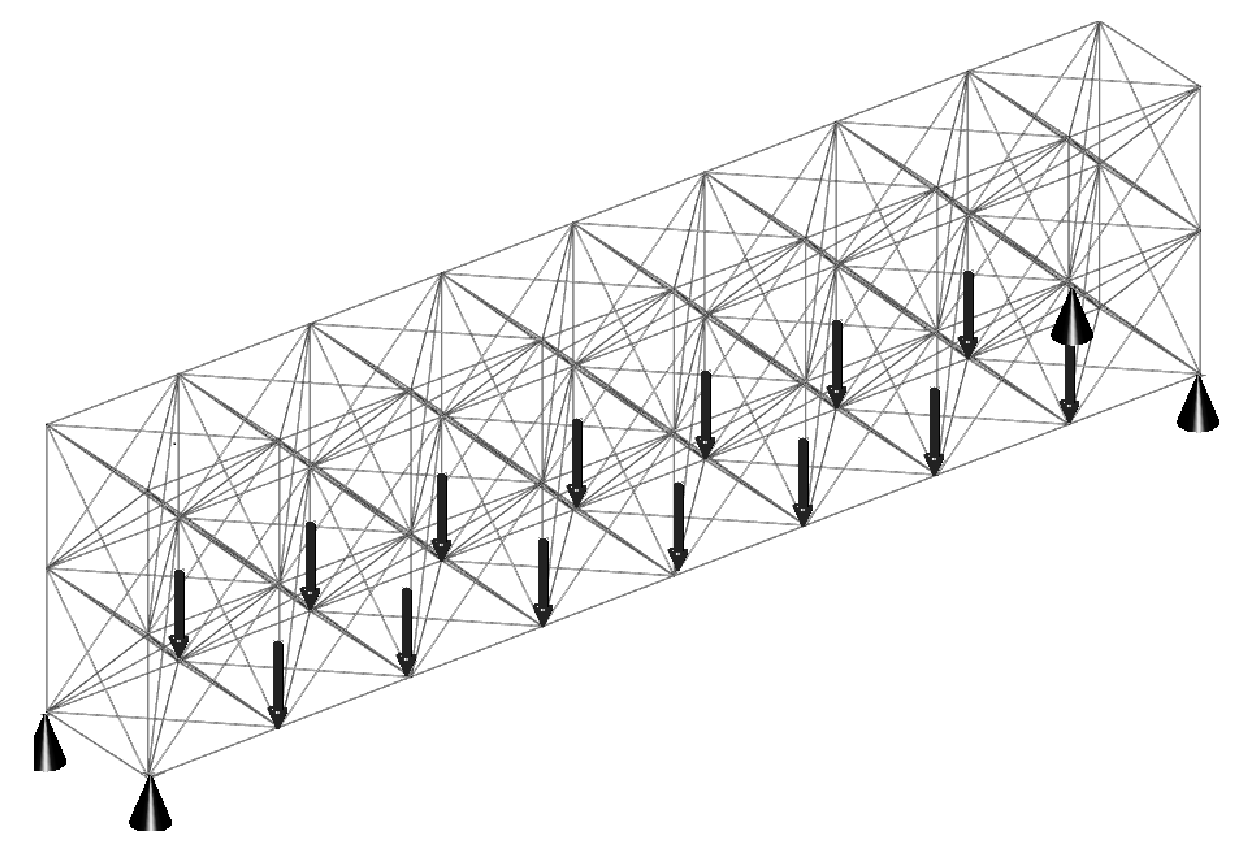
\includegraphics[scale=.2]{fig/ipnsdp_d}
  \caption{Loading condition.\\\mbox{}}
  \label{fig:design}
\end{subfigure}
\begin{subfigure}{.34\textwidth}
\centering
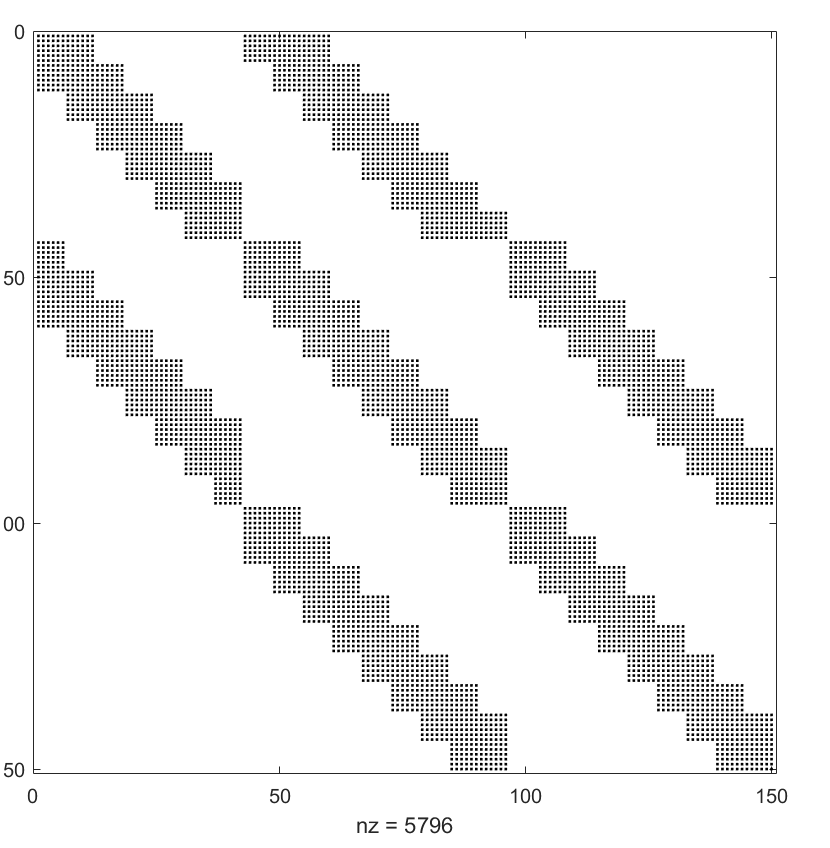
\includegraphics[scale=.2]{fig/D1}
  \caption{Sparsity of $K(a,v)+\tau G(a,v,u)$.\\(Before completion for chordality)}
  \label{fig:sp}
\end{subfigure}
\begin{subfigure}{.3\textwidth}
\centering
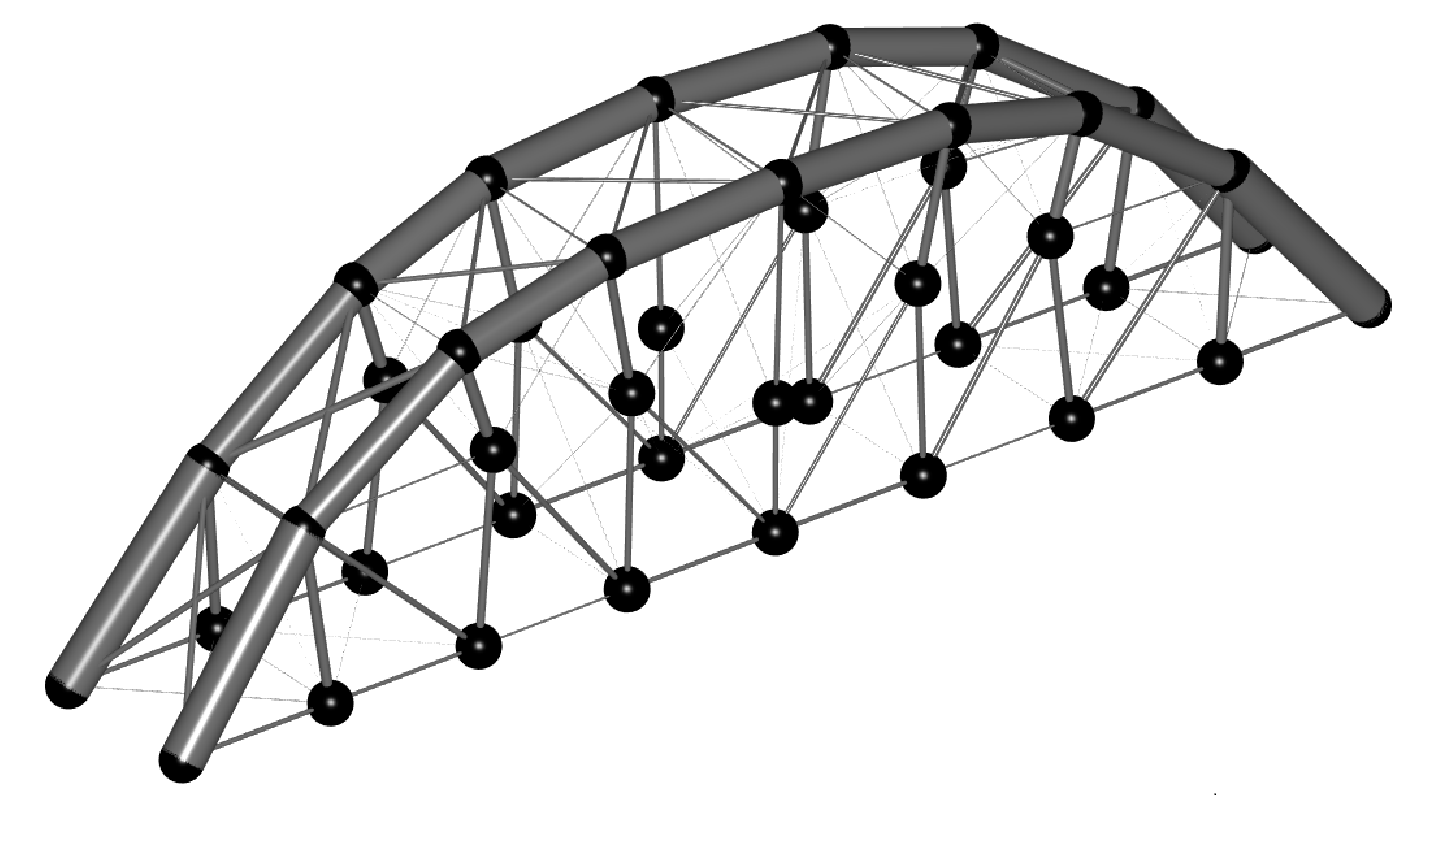
\includegraphics[scale=.2]{fig/ipnsdp_o}
  \caption{Optimal design.\\ \mbox{}}
  \label{fig:opt}
\end{subfigure}
\caption{Example~\ref{eg:topgeo} – Loading condition, sparsity pattern of the resulting matrix, and optimal design.}
\label{fig:topgeo}
\end{figure*}

The results are presented in Table~\ref{tab:chord_eff}. The table also illustrates the efficiency of the decomposition, showing that the computational time per iteration was reduced by a factor of approximately 53. This improvement was achieved by completing for chordality and  decomposing the $150 \times 150$ matrix in Figure~\ref{fig:sp} into 8 blocks, each of size between 30 and 36. Note that this problem was previously solved in~\cite{Weldeyesus2024}, where the derivatives were computed manually and the chordal decomposition was performed in advance, not by the solver. In contrast, in this paper, the derivatives are obtained via automatic differentiation, and the decomposition is carried out using the built-in feature of IPNSDP. The complete code for this example is provided in \texttt{t\_buckgeo.m}.
\begin{table}
\centering
\caption{Computational results and comparison of solution times with and without chordal decomposition for Example~\ref{eg:topgeo}. A single $150 \times 150$ matrix was decomposed into 8 blocks of size between 30 and 36.}

\begin{tabular}{lll|lll}
\toprule
\multicolumn{3}{c|}{Without chordal decomposition} & \multicolumn{3}{c}{With chordal decomposition} \\
\midrule
f\_val & IPM iter & CPU (s) & f\_val & IPM iter & CPU (s) \\
\midrule
4.3368 & 86 & 3166 & 4.3373 & 64 & 44 \\
\bottomrule
\end{tabular}\label{tab:chord_eff}
\end{table}
\end{example}

\begin{example}\label{eg:logistic_sdp}
This example presents a financial model that can be applied to classify failing and non-failing companies. The model is based on a Logit framework with a positive semidefinite quadratic discriminant function. A similar learning problem has been studied in~\cite{IPMSDP_2012}. The objective is to maximize the following function:
\begin{equation} \label{eq:logistic_sdp}
\begin{aligned}
\max_{Q} \quad & \sum_{i=1}^{M} \left( y_i z(x_i) - \log\left(1 + e^{z(x_i)}\right) \right) \\
\text{subject to} \quad & Q \succeq 0,
\end{aligned}
\end{equation}
where, the parameters (variables) to be optimized are \( a \in \mathbb{R} \), \( b \in \mathbb{R}^q \), and \( Q \in \mathbb{S}^q \). The function \( z(x) \) is defined as
\[
z(x) = a + b^T x + \frac{1}{2} x^T Q x
\]
Here, \( x_i \in \mathbb{R}^q \) represents the financial data for company \( i \), and \( y_i \in \{0, 1\} \) is a binary indicator (\( y_i = 0 \) for non-failure, \( y_i = 1 \) for failure). In practice, this problem involves a large number of learning data \( M \) and a small number of features \( q \). Although the problem is nonlinear and potentially prone to numerical instability due to the exponential term in the objective function, the number of the optimization variables is relatively small, and the problem can typically be solved in a few seconds. However, for significantly large values of \( M \), the setup phase in CasADi, can take minutes.  For the numerical experiments, the entries of matrix $M$ are generated from standard normal data adjusted using random average and spread vectors and then normalized between 0 and 1. See Table~\ref{tab:logistic_sdp} for computational results. Note that for this example a 'separate' step strategy was used to determine the step length for the search directions.  The complete code for this example is included in \texttt{f\_d.m} in the distribution of the solver.
\begin{table}
\centering
\caption{Computational results for Example~\ref{eg:logistic_sdp}.}
\begin{tabular}{ccc}
\toprule
Sizes $(M,q)$ & IPM iter & CPU (s) \\
\midrule
(12,000,6)  & 21 & <1 \\
(12,000,8)   & 19 & 3 \\
(12,000,10)   & 46 & 13 \\
(12,000,12)   & 27 & 13 \\
\bottomrule
\end{tabular}\label{tab:logistic_sdp}
\end{table}

\end{example}
\begin{example}\label{eg:bmi}
This example is adapted from~\cite{M_stingleTheis_2006}. It involves a bilinear matrix inequality and is formulated as
\begin{equation}
\begin{aligned}
    \min_{x \in \mathbb{R}^n,\, \lambda \in \mathbb{R}} \quad & \lambda \\
    \text{s.t.} \quad 
    & -|c^\ell| \leq x^\ell \leq |c^\ell|, \quad \ell = 1, \dots, n, \\
    & B(x) = A_0 + \sum_{k=1}^n x_k A_k + \sum_{i=1}^d \sum_{j=1}^d x_i x_j K_{i,j} \preceq \lambda I_m,
\end{aligned}
\tag{11.1}
\end{equation}
where \(A_k \in \mathbb{S}^m\) for \(k = 0, \dots, n\), \(K_{i,j} \in \mathbb{S}^m\) for \(i,j = 1, \dots, d\), and \(0 < d \leq n\). The bounds \(c^\ell\), \(\ell = 1, \dots, n\), and the entries of the matrices \(A_k\) and \(K_{i,j}\) are randomly drawn from the standard normal distribution. All matrices are approximately 20\% dense; however, the aggregated matrix \(B(x)\) is fully dense (100\%), which makes the problem unsuitable for chordal decomposition, particularly in this setting. However, if \(B(x)\) possesses a structured sparsity pattern, likely arising from specific applications, such problems could potentially be solved efficiently by IPNSDP. The numerical results are presented in Table~\ref{tab:bmi}. The implementation is provided in \texttt{bmi\_1.m}, included in the solver distribution.
\begin{table}
\centering
\caption{Computational results for Example~\ref{eg:bmi}.}
\begin{tabular}{ccc}
\toprule
Sizes $(n,d,m)$ & IPM iter & CPU (s) \\
\midrule
(50,25,50)  & 25& 6 \\
(50,50,50)   & 28 & 7 \\
(100,50,100)   & 28 & 99\\
(100,100,100)   & 33 & 162 \\
\bottomrule
\end{tabular}\label{tab:bmi}
\end{table}
%\end{example}


\end{example}

\begin{example}\label{eg:guass}
In this example, a problem known by a Gaussian channel capacity problem is solved. This has been solved in~\cite{IPMSDP_2012, Yamakawa_2022}. It is formulated as 
\begin{align*}
& \underset{x_i, t_i}{\text{minimize}}
& & \frac{1}{2}\sum_{i=1}^{n}\log(1+t_i) \\
& \text{subject to}
& & \frac{1}{n}\sum_{i=1}^{n}x_i\le 1 \\
& & & x_i\ge 0, \quad t_i\ge 0, \quad i=1,\dots,n \\
& & & \begin{bmatrix}
1-a_it_i & \sqrt{r_i} \\
\sqrt{r_i} & a_ix_i+r_i
\end{bmatrix} \succeq 0, \quad i=1,\dots,n.
\end{align*}
The problem features a nonlinear objective function and a large number \( n \) of linear matrix inequality constraints, each of dimension \( 2 \times 2 \). Due to the relatively small size of these matrix inequalities, the problem can be efficiently solved for larger instances compared to the other examples discussed in this report. For example, a problem involving $3200$ such matrices was solved in under two minutes. For the results reported in Table~\ref{tab:gauss}, the parameters \( r_i \) and \( a_i \), for \( i = 1, \ldots, n \), are randomly generated within the interval \([0,1]\). The implementation code is provided in \texttt{g\_c\_cap.m}.
 
\begin{table}
\centering
\caption{Computational results for Example~\ref{eg:guass}.}
\begin{tabular}{ccc}
\toprule
Number of matrices $n$ & IPM iter & CPU (s) \\
\midrule
100  & 24& <1\\
200   & 27 & <1 \\
400   & 27& 2 \\
800  & 31 & 6 \\
1600  & 33 & 20 \\
3200  & 35 & 74 \\
\bottomrule
\end{tabular}\label{tab:gauss}
\end{table}
\end{example}

\begin{remark}
  The IPNSDP software distribution includes additional examples, such as positive semidefinite programming extensions of selected test cases from the Hock and Schittkowski libraries~\cite{HockSchittkowski1981} for testing nonlinear programming solvers and widely used in the NSDP literature~\cite{penlab, IPMSDP_2012},  the minimization of the minimum eigenvalue problem, and  the primal and dual formulations of the well-known matrix completion problem.
\end{remark}

\begin{remark}
In general, IPNSDP obtains solutions within a reasonable number of iterations when the problems exhibit convexity and when it is provided with feasible initial points. Although it includes features such as scaling and checks for linear constraint feasibility, it is still recommended to supply a feasible initial point. Furthermore, for some problems, performance can be improved by customizing the algorithmic settings or the penalization strategy through its options.
\end{remark}

\section{Conclusion}\label{sec:conc}
The paper introduces IPNSDP, an alternative MATLAB solver designed to address Nonlinear Semidefinite Programming (NSDP) problems using a second-order interior point method. IPNSDP aims to simplify the user experience by integrating with \textsc{CasADi} for automatic differentiation, thereby reducing the manual effort typically required for derivative computations involving matrix calculus.

For large-scale problems with structured sparse matrix constraints, IPNSDP leverages a chordal decomposition technique. This approach decomposes a single large positive semidefinite constraint into multiple smaller ones, significantly improving computational efficiency. To further improve the efficiency, the solver applies a clique merging strategy that combines submatrices with substantial overlap. This procedure is particularly beneficial for applications such as structural optimization, where these problem structures frequently occur.

Additionally, IPNSDP provides customization options for both the interior point algorithm and the decomposition procedures, enabling users to fine-tune the solver’s performance. Overall, IPNSDP offers a practical and user-friendly framework that combines advanced algorithmic strategies with automated tools to effectively solve a wide class of NSDPs.

\section*{Acknowledgement}
We thank the School of Mathematics and the Maxwell Institute for Mathematical Sciences at the University of Edinburgh for providing institutional support and hosting for the project.

%\begin{verbatim}
\bibliographystyle{tfs}
\bibliography{interacttfssample}
%\end{verbatim}




% Appendix
\appendix
\section{Complete IPNSDP Problem Setup Template}
\label{app:template}

\lstset{
  language=Matlab,
  basicstyle=\ttfamily\small,
  breaklines=true,
  frame=single,
  columns=flexible,
  captionpos=b,
  numbers=left,
  numberstyle=\tiny,
  stepnumber=1,
  numbersep=5pt
}

\lstinputlisting[caption={\texttt{ipnsdp\_user\_template.m} -- user input template for IPNSDP},label={lst:template}]{ipnsdp_user_template.m}
\end{document}
